\documentclass[11pt]{article}
\usepackage{../EllioStyle}
\usepackage{listings}

\definecolor{codegreen}{rgb}{0,0.6,0}
\definecolor{codegray}{rgb}{0.5,0.5,0.5}
\definecolor{codepurple}{rgb}{0.58,0,0.82}
\definecolor{backcolour}{rgb}{0.95,0.95,0.92}

\lstdefinestyle{mystyle}{
%    backgroundcolor=\color{backcolour},   
    commentstyle=\color{codegreen},
    keywordstyle=\color{magenta},
    numberstyle=\tiny\color{codegray},
    stringstyle=\color{codepurple},
    basicstyle=\ttfamily\footnotesize,
    breakatwhitespace=false,         
    breaklines=true,                 
    captionpos=b,                    
    keepspaces=true,                 
    numbers=left,                    
    numbersep=5pt,                  
    showspaces=false,                
    showstringspaces=false,
    showtabs=false,                  
    tabsize=2
}

\title{Homework 3}
\author{Elliott Pryor}
\date{24 October 2021}

\rhead{Homework 3}

\begin{document}
\maketitle

\problem{2}

By hand, build an FM-index for S = gacgaacgac\$. You may report the BW[], C[] and occ[ , ] data structures as simple tables.

\hrule

For our reference, we give the suffix array so it is easier for us to build the FM-index by hand.
We list all the suffixes: 





gacgaacgac\$,
acgaacgac\$,
cgaacgac\$,
gaacgac\$,
aacgac\$,
acgac\$,
cgac\$,
gac\$,
ac\$,
c\$,
\$

\begin{table}[h]
    \centering
    \begin{tabular}{| c | c | l | c |}
        \hline
        $i$ & SA & Suffix & BW[i] \\ \hline
        1 & 11 & \$ & c \\
        2 & 5 & aacgac\$ & g \\
        3 & 9 & ac\$ & g \\
        4 & 2 & acgaacgac\$ & g \\
        5 & 6 & acgac\$ & a \\
        6 & 10 & c\$ & a \\
        7 & 3 & cgaacgac\$ & a \\
        8 & 7 & cgac\$ & a \\
        9 & 4 & gaacgac\$ & c \\
        10 & 8 & gac\$ & c \\
        11 & 1 & gacgaacgac\$ & \$ \\ \hline
    \end{tabular}
    \caption{The last column is the BW[] for the FM-Index}
\end{table}

\begin{table}[h]
    \centering
    \begin{tabular}{| c | c |}
        \hline
        Letter & Count \\ \hline
        \$ & 0 \\
        a & 1 \\
        c & 5 \\
        g & 8 \\ \hline
    \end{tabular}
    \caption{C[] for the FM-Index}
\end{table}

\begin{table}[h]
    \centering
    \begin{tabular}{| c | c | c | c | c |}
        \hline
        $i$  & \$ & a & c & g \\ \hline
            1 & 0 & 0 & 1 & 0 \\
            2 & 0 & 0 & 1 & 1 \\
            3 & 0 & 0 & 1 & 2 \\
            4 & 0 & 0 & 1 & 3 \\
            5 & 0 & 1 & 1 & 3 \\
            6 & 0 & 2 & 1 & 3 \\
            7 & 0 & 3 & 1 & 3 \\
            8 & 0 & 4 & 1 & 3 \\
            9 & 0 & 4 & 2 & 3 \\
            1 & 0 & 4 & 3 & 3 \\
            1 & 1 & 4 & 3 & 3 \\ \hline
    \end{tabular}
    \caption{occ table for the FM-Index}
\end{table}

\problem{3}
Trace the backwards search algorithm to determine if the pattern Q = gac belongs to S = gacgaacgac\$.

\hrule

\begin{enumerate}[\text{Iteration} 1:]
    \item 
    st = 1,
    ed = 11,
    i = 3 \\
    x = c,
    st' = C[c] + occ(c, 0) + 1 = 6,
    ed' = C[c] + occ(c, 11) = 8

    \item
    st = 6,
    ed = 8,
    i = 2 \\
    x = a,
    st' = C[a] + occ(a, 5) + 1= 3,
    ed' = C[a] + occ(a, 8) = 5

    \item
    st = 3,
    ed = 5,
    i = 1 \\
    x = g
    st' = C[g] + occ(g, 2) + 1 = 10,
    ed' = C[g] + occ(g, 5) = 11

    \item Output 2 matches at 10, 11
\end{enumerate}

\problem{1}
Write a program to compute the suffix array for a given input string.
You can either prompt the user for a string, or use a command-line argument to specify the string.
Demonstrate it works on a few strings.

Then, use your program to find the suffix array for the string S = gacgaacgac\$.
\hrule

\begin{figure}[h] 
    \centering
    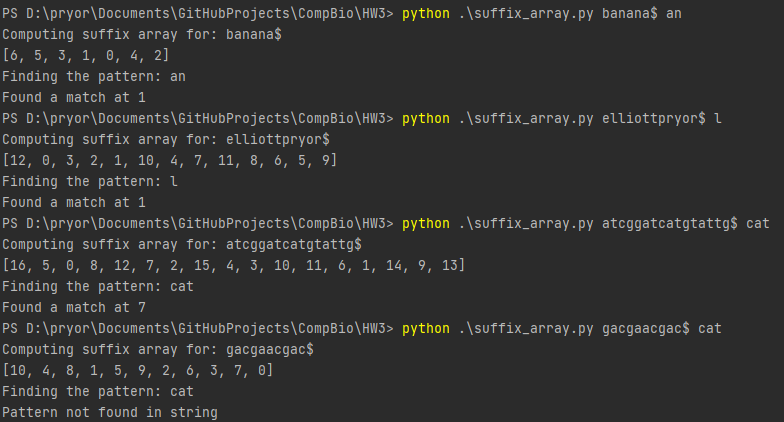
\includegraphics[width=0.9 \linewidth]{examples.png}
    \label{fig:examples}
    \caption{Examples showing that my program works. I also implemented the bonus and a query
    string is provided for all examples.
    Also note the last example is the one that we were asked to provide.
    Please note that I use 0-indexing.}
\end{figure}

\lstset{style=mystyle}
\lstinputlisting[language=Python]{suffix_array.py}



\end{document}